\documentclass[UTF8,a4paper,12pt]{ctexart}

% 基础宏包
\usepackage{geometry}
\geometry{left=2.5cm, right=2.5cm, top=2.5cm, bottom=2.5cm}
\usepackage{graphicx}
\usepackage{amsmath}
\usepackage{float}
\usepackage{caption}

% 字体设置
\setCJKmainfont{SimSun}[AutoFakeBold=true,AutoFakeSlant=true]  % 宋体正文

% 设置标题字体为楷体（自动检测系统字体或本地字体）
\IfFontExistsTF{KaiTi}{
    \newCJKfontfamily\kaiti{KaiTi}[AutoFakeBold=true]
}{
    \IfFontExistsTF{SimKai}{
        \newCJKfontfamily\kaiti{SimKai}[AutoFakeBold=true]
    }{
        \IfFileExists{font/SIMKAI.TTF}{
            \newCJKfontfamily\kaiti{font/SIMKAI.TTF}[AutoFakeBold=true]
        }{
            \newCJKfontfamily\kaiti{SimSun}[AutoFakeBold=true]
        }
    }
}

% 英文用 Times New Roman
\setmainfont{Times New Roman}

% 段落设置
\setlength{\parindent}{2em}
\setlength{\parskip}{0pt}

% 字号定义
\newcommand{\sihao}{\fontsize{14pt}{16.8pt}\selectfont}      % 四号

% 去掉页码
\pagestyle{empty}

% 图计数器（手动编号）
\newcounter{figcounter}
\setcounter{figcounter}{0}
\newcommand{\figcaption}{\stepcounter{figcounter}\par\vspace{0.3em}\noindent\hspace*{\fill}\textbf{图\thefigcounter}\hspace*{\fill}}

% 自定义章节标题格式
\newcommand{\patentsection}[1]{\par\vspace{0.5em}\noindent{\kaiti\bfseries #1}\par\vspace{0.3em}}

% ============ 文档开始 ============
\begin{document}

% 顶部居中标题
\begin{center}
    {\kaiti\sihao\bfseries 专利申请技术交底书}
\end{center}

\vspace{1em}

\patentsection{技术联系人：********}

\patentsection{技术联系电话：********}

\patentsection{电子邮件：********}

\patentsection{1、发明名称}

一种结合CNN迁移学习和SVDD的图像异常检测方法

\patentsection{2、背景技术}

描述发明人所知的与本发明技术方案相近的已有技术，并描述已有技术有何缺点，对其存在的问题或不足进行评述；如有引证文献，请一一列出。

高铁接触网系统作为列车的重要部分，其运行状况对列车的安全有至关重要的影响。接触网支柱编号的状态检测作为接触网支柱编号识别前的重要工作步骤，对接触网支柱编号的异常检测不仅可以快速判定道路安全信息，也可以为高速铁路管理提供极大的便利。

传统通过图像和模式识别进行异常检测的方法是通过适应于检测对象的固定算法或者人工确定并提取相应特征，再通过异常检测算法进行异常检测。这类方法往往需要大量的样本和特征信息，不能很好地针对不平衡数据。而在异常检测中异常类数据的获取往往需要大量的人力物力，并且在实际中异常类数据相对很少，采用异常检测可能效果不佳。第二是通过人工确定的特征不能准确地反映图像的深度特征表达。

\patentsection{3、发明创造所要解决的技术问题及发明目的}

针对现有技术的缺点，提出本专利要解决的技术问题，技术问题有多个时，请按重要性排序，并列出本发明的主要目的，可结合技术方案加以说明。

本发明所要解决的技术问题是提供一种结合CNN（卷积神经网络）迁移学习和SVDD（Support Vector Data Description，支持向量数据描述）的图像异常检测方法，解决现有异常检测方法存在的提取图像特征信息不准确、不能很好地解决非平衡数据的技术问题，有效地实现高速列车接触网图像异常检测。

\patentsection{4、清楚完整的叙述发明创造的技术方案}

通过Model2判断测试样本与超球体的关系，最终判断测试样本是否异常。

通过之前训练好的Model1对测试样本进行特征提取，其次将提取到的特征数据作为SVDD分类器的测试样本，通过比较测试样本和正常域模型的关系，得到最终测试样本是否异常。通过相关实验，能够很好地判断接触网支柱编号数据是否属于异常。

\patentsection{5、与现有技术相比，本发明所具有的优点，例如数据安全、网络资源节省等，最好是结合关键技术方案进行说明如何会产生良好的技术效果。}

与现有技术相比，本发明的有益效果是：1)有效利用列车视频设备，视频信息量更丰富，简单方便，不受机车车型影响，各种车型都可使用。2)能够很好地处理传统方法中需要人为确定特征及处理非平衡数据中异常类数据少等问题。3)自动化处理水平较高，可以极大地降低操作人员工作量，及早发现接触网支柱编号异常问题，提高巡检效率。

\patentsection{6、附图及说明}

\patentsection{通信方法类请给出流程图；系统或装置类请给出结构图、电路图或原理框图；附图要写明图名，并提供可编辑格式的电子档，以便代理人编辑修改。}

注意：请提供可编辑形式的附图。

图1为本发明实施例中使用的改进的Lenet-5网络结构图。

图2为本发明一种结合CNN迁移学习和SVDD的图像异常检测方法流程图。

% 图1
\begin{center}
    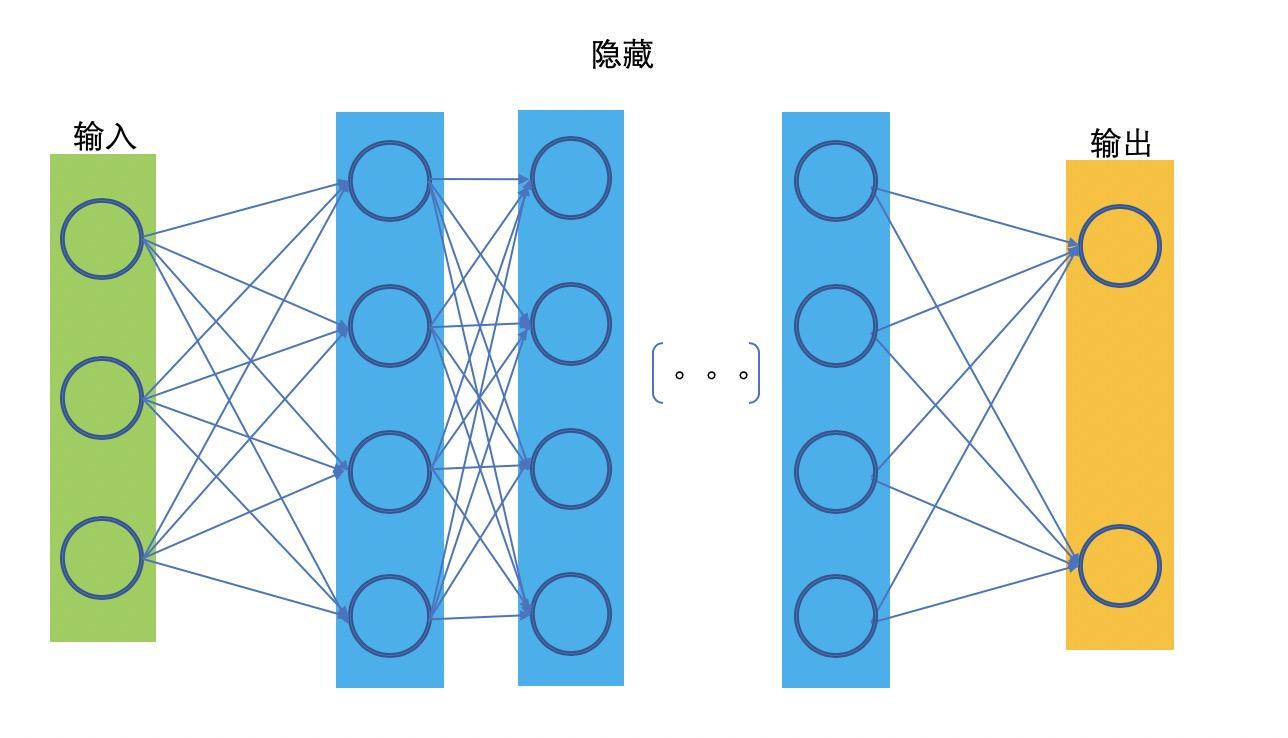
\includegraphics[width=0.9\textwidth]{figture/example.jpg}
\end{center}
\figcaption

% 图2
\begin{center}
    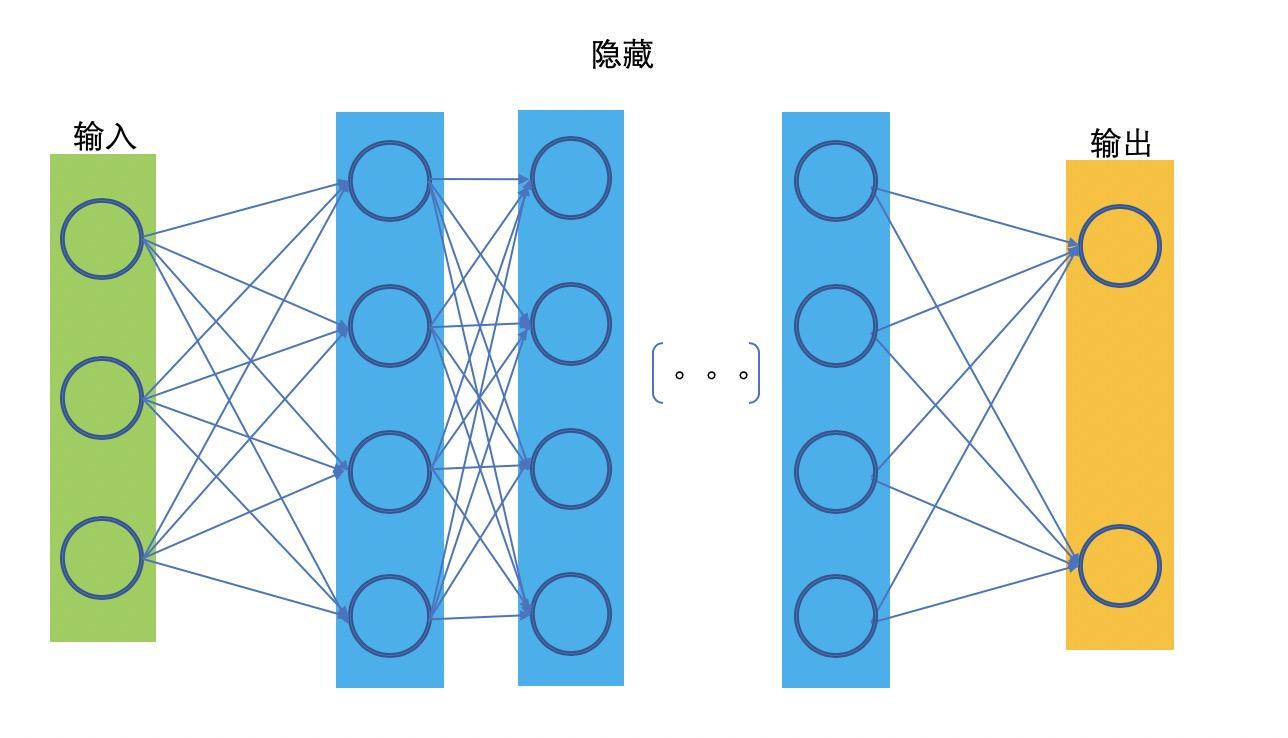
\includegraphics[width=0.9\textwidth]{figture/example.jpg}
\end{center}
\figcaption

\end{document}
